\section{基于测试函数的比较}
\label{sec:dcomp-ipm}

密度比较要求两个分布写在同一个支配测度下，并且只看同一位置上的取值。另一种做法不碰密度，只看两个分布对一些函数给出的平均。选定一个函数$g$，读出$\mathbb{E}_{P}[g]$与$\mathbb{E}_{Q}[g]$，两者的差就是用$g$这把“尺子”量到的差异。用一族尺子同时去量，取最大的读数差，就得到一个比较量。式~\eqref{eq:dcomp-tv-dual}已经是这种形式：总变差是有界函数单位球上的最大期望差。这里要回答的是：换成别的函数类会得到什么，函数类要多丰富才能分辨所有不同的分布，以及怎样实际算出上确界。

\subsection{函数类与可辨别差异}
\label{sec:dcomp-ipm-classes}

\begin{definition}[积分概率度量]
\label{def:dcomp-ipm}
设$\mathcal{G}$是一族$\mathcal{X}$上的实值可测函数，其中每个$g$在$P$与$Q$下都可积。称
\begin{equation}
 d_{\mathcal{G}}(P,Q)=\sup_{g\in\mathcal{G}}\bigl\lvert\mathbb{E}_{P}[g]-\mathbb{E}_{Q}[g]\bigr\rvert
 \label{eq:dcomp-ipm-def}
\end{equation}
为由$\mathcal{G}$生成的\term{积分概率度量}（integral probability metric）。
\end{definition}

这个量对称，并且满足三角不等式：对第三个分布$R$与每个$g$，
\[
 \lvert\mathbb{E}_{P}g-\mathbb{E}_{R}g\rvert\leq\lvert\mathbb{E}_{P}g-\mathbb{E}_{Q}g\rvert+\lvert\mathbb{E}_{Q}g-\mathbb{E}_{R}g\rvert ,
\]
再对$g$取上确界。定义要检查两件事。

第一，上确界是否有限。若$\mathcal{G}$对数乘封闭，例如取全体有界可测函数而不限制大小，只要某个$g$的读数差不为零，把$g$放大$c$倍读数差就放大$c$倍，上确界是$+\infty$。所以函数类通常要带一个范数约束，如$\lVert g\rVert_{\infty}\leq1$。

第二，零值能否辨别分布。比较量为零只说明$P$与$Q$在$\mathcal{G}$中每个函数上的平均相同。若$\mathcal{G}$太小，不同的分布也可能得到零。取$\mathcal{G}$只含$x$与$x^{2}$两个函数，它只比较均值与二阶矩。标准高斯分布$P$与区间$(-\sqrt3,\sqrt3)$上的均匀分布$Q$的均值都是$0$，二阶矩都是$1$，所以这个函数类给出的比较量为零，两个分布却明显不同，见图~\ref{fig:dcomp-moment-matching}。一旦加入$\cos x$或$\mathbf{1}_{\{\lvert x\rvert\leq1\}}$这样的函数，差异立即显现：
\[
 \mathbb{E}_{P}[\cos X]-\mathbb{E}_{Q}[\cos X]=\mathrm{e}^{-1/2}-\frac{\sin\sqrt3}{\sqrt3}\approx0.0367,
\]
\[
 P(\lvert X\rvert\leq1)-Q(\lvert X\rvert\leq1)=\bigl(2\Phi(1)-1\bigr)-\frac{1}{\sqrt3}\approx0.1053 .
\]

\begin{BookInlineFigure}
 \centering
 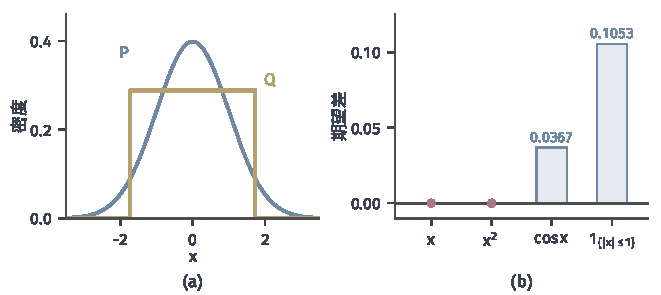
\includegraphics[width=112mm]{figures/07-probability/04-distribution-analysis/matplotlib/dcomp-moment-matching/figure.pdf}
 \caption{函数类决定能看到的差异。(a)$P=\mathcal{N}(0,1)$（蓝）与$Q=\operatorname{Unif}(-\sqrt3,\sqrt3)$（黄），均值都是$0$，方差都是$1$。(b)四个测试函数上的期望差$\mathbb{E}_{P}[g]-\mathbb{E}_{Q}[g]$：$x$与$x^{2}$为零（红点），$\cos x$与$\mathbf{1}_{\{\lvert x\rvert\leq1\}}$不为零。}
 \label{fig:dcomp-moment-matching}
\end{BookInlineFigure}

几种常见的函数类各有含义。有界函数单位球给出$2d_{\mathrm{TV}}$，能辨别任何两个不同的分布，但对位置的微小移动同样“看得见”，见第~\ref{sec:dcomp-tv-definition}节末尾。$\mathbb{R}$上半直线的示性函数$\mathbf{1}_{(-\infty,t]}$给出$\sup_t\lvert F_P(t)-F_Q(t)\rvert$，称为\term{Kolmogorov距离}（Kolmogorov distance）；分布函数决定分布，所以它也能辨别分布。$\mathbb{R}^{d}$上的全体有界连续函数也能辨别分布，这是第~\ref{chap:weak-convergence-of-distributions}章中弱收敛极限唯一的依据。1-Lipschitz函数类给出第~\ref{sec:dcomp-wasserstein}节的一阶Wasserstein距离。

函数类越大，比较越严格，但上确界也越难计算：对一般的函数类，要在无穷维集合上求最大值。下面构造一类函数，使上确界有闭式解。

\subsection{核均值}
\label{sec:dcomp-kernel-mean}

取再生核Hilbert空间（RKHS）的单位球作为函数类。设$k$是$\mathcal{X}$上的正定核，$\mathcal{H}$是它的RKHS，内积记作$\langle\cdot,\cdot\rangle_{\mathcal{H}}$。卷四给出了它的基本性质：每个$x$对应一个函数$k(x,\cdot)\in\mathcal{H}$，并且对一切$g\in\mathcal{H}$，
\begin{equation}
 g(x)=\bigl\langle g,\,k(x,\cdot)\bigr\rangle_{\mathcal{H}},\qquad\bigl\lVert k(x,\cdot)\bigr\rVert_{\mathcal{H}}=\sqrt{k(x,x)},
 \label{eq:dcomp-reproducing}
\end{equation}
可参考\BookChapterRef{chap:rkhs}{卷四第23章“再生核Hilbert空间”}。映射$x\mapsto k(x,\cdot)$是特征映射，它把$\mathcal{X}$中的点放进Hilbert空间。为避免与概率核混淆，本节的核用小写$k$。

再生性质~\eqref{eq:dcomp-reproducing}把求值变成内积。若在两边对$X\sim P$取期望，并把期望移进内积里，就得到
\[
 \mathbb{E}_{P}[g(X)]=\bigl\langle g,\ \mathbb{E}_{P}[k(X,\cdot)]\bigr\rangle_{\mathcal{H}} .
\]
右边的$\mathbb{E}_{P}[k(X,\cdot)]$是特征点的平均位置，也就是把单位质量按$P$放到这些特征点上之后的重心。下面的定理说明这个重心在什么条件下存在，并绕开“向量值期望”的定义，直接用内积刻画它。

\begin{theorem}[核均值]
\label{thm:dcomp-kernel-mean}
设$\mathcal{H}$可分，特征映射$x\mapsto k(x,\cdot)$可测，并且
\begin{equation}
 \mathbb{E}_{P}\Bigl[\sqrt{k(X,X)}\Bigr]<\infty .
 \label{eq:dcomp-kernel-moment}
\end{equation}
则每个$g\in\mathcal{H}$在$P$下可积，并且存在唯一的$m_P\in\mathcal{H}$，使
\begin{equation}
 \mathbb{E}_{P}[g(X)]=\langle g,m_P\rangle_{\mathcal{H}},\qquad g\in\mathcal{H} .
 \label{eq:dcomp-kernel-mean}
\end{equation}
它的取值是$m_P(y)=\mathbb{E}_{P}[k(X,y)]$。
\end{theorem}

\begin{proof}
对$g\in\mathcal{H}$，$g(x)=\langle g,k(x,\cdot)\rangle_{\mathcal{H}}$是连续线性泛函与可测映射的复合，所以$g$可测。由Cauchy--Schwarz不等式与式~\eqref{eq:dcomp-reproducing}，
\[
 \lvert g(x)\rvert\leq\lVert g\rVert_{\mathcal{H}}\sqrt{k(x,x)} .
\]
由条件~\eqref{eq:dcomp-kernel-moment}，$g$在$P$下可积，并且线性泛函$L(g)=\mathbb{E}_{P}[g(X)]$满足
\[
 \lvert L(g)\rvert\leq\mathbb{E}_{P}\Bigl[\sqrt{k(X,X)}\Bigr]\,\lVert g\rVert_{\mathcal{H}},
\]
是有界线性泛函。由Riesz表示定理，存在唯一的$m_P\in\mathcal{H}$使$L(g)=\langle g,m_P\rangle_{\mathcal{H}}$，可参考\BookChapterRef{chap:function-inner-product-spaces}{卷四第12章“内积空间”}。取$g=k(y,\cdot)$，由式~\eqref{eq:dcomp-reproducing}，左边是$\mathbb{E}_{P}[k(X,y)]$，右边是$m_P(y)$。
\end{proof}

$m_P$称为$P$的\term{核均值}（kernel mean embedding），映射$P\mapsto m_P$把概率分布表示为$\mathcal{H}$中的元素。可分性在这里的作用是保证可测性在两种意义下一致：可分Hilbert空间中，“每个$g(x)=\langle g,k(x,\cdot)\rangle$都可测”与“特征映射作为Hilbert空间值映射可测”是等价的，所以定理的条件可以按任一种理解检查。条件~\eqref{eq:dcomp-kernel-moment}是特征点到原点距离的一阶矩，有界核（如高斯核，$k(x,x)=1$）对任何分布都满足它。这一节新增的只是“分布的表示”，RKHS本身仍是卷四的对象。

\paragraph{例表上的核均值}
在例表上取$\sigma=1$的高斯核$k(x,y)=\exp(-(x-y)^{2}/2)$。分布有限时期望就是加权和，
\[
 m_P=\sum_{i}p_i\,k(x_i,\cdot)=0.6\,k(0,\cdot)+0.3\,k(1,\cdot)+0.1\,k(2,\cdot) .
\]
它是三个以$0,1,2$为中心的高斯隆起按概率加权之和，见图~\ref{fig:dcomp-kernel-mean}(a)中的点线。在三个支撑点上，
\[
 m_P(0)\approx0.7955,\qquad m_P(1)\approx0.7246,\qquad m_P(2)\approx0.3632,
\]
\[
 m_Q(0)\approx0.5361,\qquad m_Q(1)\approx0.7246,\qquad m_Q(2)\approx0.6226 .
\]
核均值是概率质量用核“抹开”后的形状。$P$的质量偏左，$m_P$的峰也偏左。

\subsection{MMD}
\label{sec:dcomp-mmd}

有了核均值，RKHS单位球上的最大期望差就是一个Hilbert空间中的最大内积问题，答案由Cauchy--Schwarz不等式直接给出。

\begin{theorem}[MMD的表示]
\label{thm:dcomp-mmd}
设$P,Q$都满足条件~\eqref{eq:dcomp-kernel-moment}。则
\begin{equation}
 \operatorname{MMD}_k(P,Q)=\sup_{\lVert g\rVert_{\mathcal{H}}\leq1}\bigl\lvert\mathbb{E}_{P}[g]-\mathbb{E}_{Q}[g]\bigr\rvert=\lVert m_P-m_Q\rVert_{\mathcal{H}} .
 \label{eq:dcomp-mmd-def}
\end{equation}
设$X,X'\sim P$，$Y,Y'\sim Q$，四者相互独立，则
\begin{equation}
 \operatorname{MMD}_k^{2}(P,Q)=\mathbb{E}\bigl[k(X,X')\bigr]-2\,\mathbb{E}\bigl[k(X,Y)\bigr]+\mathbb{E}\bigl[k(Y,Y')\bigr] .
 \label{eq:dcomp-mmd-kernel}
\end{equation}
\end{theorem}

\begin{proof}
由式~\eqref{eq:dcomp-kernel-mean}，
\[
 \mathbb{E}_{P}[g]-\mathbb{E}_{Q}[g]=\langle g,m_P-m_Q\rangle_{\mathcal{H}} .
\]
由Cauchy--Schwarz不等式，单位球上它的绝对值不超过$\lVert m_P-m_Q\rVert_{\mathcal{H}}$；若$m_P\neq m_Q$，取$m_P-m_Q$方向上的单位向量$g^{*}$即可达到，若相等则两边都是零。这证明了式~\eqref{eq:dcomp-mmd-def}。

展开平方范数，
\[
 \lVert m_P-m_Q\rVert_{\mathcal{H}}^{2}=\langle m_P,m_P\rangle_{\mathcal{H}}-2\langle m_P,m_Q\rangle_{\mathcal{H}}+\langle m_Q,m_Q\rangle_{\mathcal{H}} .
\]
对中间一项，把式~\eqref{eq:dcomp-kernel-mean}用于$g=m_P$与分布$Q$，再用$m_P(y)=\mathbb{E}_{P}[k(X,y)]$，
\[
 \langle m_P,m_Q\rangle_{\mathcal{H}}=\mathbb{E}_{Q}\bigl[m_P(Y)\bigr]=\mathbb{E}\bigl[k(X,Y)\bigr] .
\]
最后一步是对独立的$(X,Y)$用Fubini定理，所需的可积性来自$\lvert k(x,y)\rvert\leq\sqrt{k(x,x)k(y,y)}$与条件~\eqref{eq:dcomp-kernel-moment}。另两项同理。
\end{proof}

\term{最大均值差异}（maximum mean discrepancy）这个名字来自式~\eqref{eq:dcomp-mmd-def}的左端，简称MMD。达到上确界的$g^{*}$称为\term{见证函数}（witness function），它在$P$质量多于$Q$的地方取正值，在少于$Q$的地方取负值，是RKHS单位球中最能“看出”两者差别的那把尺子。式~\eqref{eq:dcomp-mmd-kernel}把无穷维的上确界化成了三个核期望：同一分布内两点的平均相似度，减去跨分布两点的平均相似度的两倍。

\paragraph{例表上的计算}
继续用$\sigma=1$的高斯核。记$\bm{K}$为$3\times3$矩阵，$\bm{K}_{i,j}=k(i-1,j-1)$，即$\exp(-(i-j)^{2}/2)$。三个核期望是二次型，
\[
 \bm{p}^{\top}\bm{K}\bm{p}\approx0.7310,\qquad\bm{p}^{\top}\bm{K}\bm{q}\approx0.6013,\qquad\bm{q}^{\top}\bm{K}\bm{q}\approx0.6272 .
\]
由式~\eqref{eq:dcomp-mmd-kernel}，
\[
 \operatorname{MMD}_k^{2}(P,Q)\approx0.7310-2\times0.6013+0.6272=0.1556 .
\]
也可以直接用$\bm{p}-\bm{q}=(0.3,0,-0.3)^{\top}$计算二次型：
\[
 (\bm{p}-\bm{q})^{\top}\bm{K}(\bm{p}-\bm{q})=0.09\,(1+1-2\mathrm{e}^{-2})=0.18(1-\mathrm{e}^{-2})\approx0.1556 .
\]
开方得$\operatorname{MMD}_k(P,Q)\approx0.3945$。见证函数在三个支撑点上的值是$0.6575$，$0$，$-0.6575$，代入
\[
 \begin{aligned}
 \mathbb{E}_{P}[g^{*}]-\mathbb{E}_{Q}[g^{*}]&=\sum_i(p_i-q_i)\,g^{*}(x_i)\\
 &=0.3\times0.6575+(-0.3)\times(-0.6575)\approx0.3945 ,
 \end{aligned}
\]
与MMD相等，见图~\ref{fig:dcomp-kernel-mean}(b)。

\begin{BookInlineFigure}
 \centering
 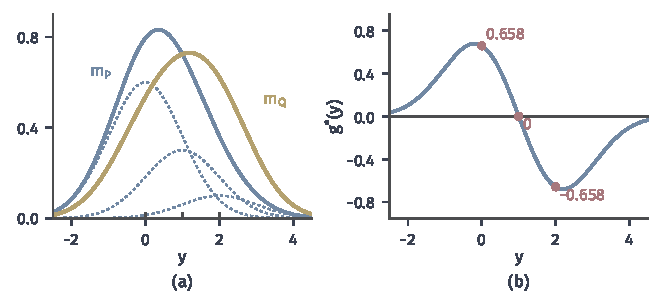
\includegraphics[width=112mm]{figures/07-probability/04-distribution-analysis/matplotlib/dcomp-kernel-mean/figure.pdf}
 \caption{例表的核均值，高斯核$\sigma=1$。(a)$m_P$（蓝）与$m_Q$（黄）；蓝色点线是三个加权核截面$p_i\,k(x_i,\cdot)$，深灰短线标出支撑点$0,1,2$。(b)见证函数$g^{*}=(m_P-m_Q)/\operatorname{MMD}_k$，红点是它在支撑点上的值。}
 \label{fig:dcomp-kernel-mean}
\end{BookInlineFigure}

式~\eqref{eq:dcomp-mmd-kernel}是两个总体分布之间的量。实际中常常只有两组样本，把期望换成样本平均就得到估计值；估计的偏差、方差与检验属于卷八的内容，这里只讨论总体量本身。

\subsection{核的辨别能力}
\label{sec:dcomp-characteristic}

MMD为零意味着$m_P=m_Q$。核均值是否把不同的分布映到不同的元素，取决于核。

\begin{definition}[特征核]
\label{def:dcomp-characteristic}
设$\mathcal{P}_k$是满足条件~\eqref{eq:dcomp-kernel-moment}的全体概率分布。若映射$P\mapsto m_P$在$\mathcal{P}_k$上是单射，则称$k$为\term{特征核}（characteristic kernel）。
\end{definition}

由式~\eqref{eq:dcomp-mmd-def}，$k$是特征核当且仅当对$\mathcal{P}_k$中的分布，$\operatorname{MMD}_k(P,Q)=0$等价于$P=Q$。不是特征核的例子很容易造。线性核$k(x,y)=xy$的RKHS只含线性函数，$m_P(y)=y\,\mathbb{E}_{P}[X]$，MMD只比较均值。二次核$k(x,y)=(1+xy)^{2}$的核均值是
\[
 m_P(y)=\mathbb{E}_{P}\bigl[(1+Xy)^{2}\bigr]=1+2y\,\mathbb{E}_{P}[X]+y^{2}\,\mathbb{E}_{P}[X^{2}],
\]
它只记录前两阶矩。图~\ref{fig:dcomp-moment-matching}中的两个分布在这个核下MMD为零。高斯核则不同。

在$\mathbb{R}^{d}$上取带宽$\sigma>0$的高斯核
\begin{equation}
 k_\sigma(\bm{x},\bm{y})=\exp\Bigl(-\frac{\lVert\bm{x}-\bm{y}\rVert_2^{2}}{2\sigma^{2}}\Bigr) .
 \label{eq:dcomp-gauss-kernel}
\end{equation}
它的谱表示把MMD与特征函数联系起来。

\begin{theorem}[高斯核的谱表示]
\label{thm:dcomp-gauss-characteristic}
设$k_\sigma$如式~\eqref{eq:dcomp-gauss-kernel}，$\Lambda_\sigma$是协方差矩阵为$\sigma^{-2}\bm{I}$的中心高斯分布。对$\mathbb{R}^{d}$上任意概率分布$P,Q$，
\begin{equation}
 \operatorname{MMD}_{k_\sigma}^{2}(P,Q)=\int_{\mathbb{R}^{d}}\bigl\lvert\phi_P(\bm{\omega})-\phi_Q(\bm{\omega})\bigr\rvert^{2}\,\Lambda_\sigma(\mathrm{d}\bm{\omega}),
 \label{eq:dcomp-mmd-spectral}
\end{equation}
其中$\phi_P,\phi_Q$是两个分布的特征函数。因此$k_\sigma$是特征核。
\end{theorem}

\begin{proof}
设$\bm{W}\sim\Lambda_\sigma$。高斯分布的特征函数给出，对任意$\bm{u}\in\mathbb{R}^{d}$，
\[
 \mathbb{E}\bigl[\mathrm{e}^{\mathrm{i}\langle\bm{W},\bm{u}\rangle}\bigr]=\exp\Bigl(-\frac{\lVert\bm{u}\rVert_2^{2}}{2\sigma^{2}}\Bigr)=k_\sigma(\bm{x},\bm{y}),\qquad\bm{u}=\bm{x}-\bm{y} .
\]
取$\bm{X}\sim P$，$\bm{Y}\sim Q$与$\bm{W}$相互独立。被积函数的模为$1$，由Fubini定理可以先对$\bm{X},\bm{Y}$积分：
\[
 \mathbb{E}\bigl[k_\sigma(\bm{X},\bm{Y})\bigr]=\mathbb{E}\Bigl[\mathbb{E}\bigl[\mathrm{e}^{\mathrm{i}\langle\bm{W},\bm{X}\rangle}\bigr]\,\overline{\mathbb{E}\bigl[\mathrm{e}^{\mathrm{i}\langle\bm{W},\bm{Y}\rangle}\bigr]}\Bigm|\bm{W}\Bigr]=\int\phi_P(\bm{\omega})\overline{\phi_Q(\bm{\omega})}\,\Lambda_\sigma(\mathrm{d}\bm{\omega}) .
\]
对$(P,P)$与$(Q,Q)$同样计算，代入式~\eqref{eq:dcomp-mmd-kernel}，三项合成$\lvert\phi_P-\phi_Q\rvert^{2}$的积分，即式~\eqref{eq:dcomp-mmd-spectral}。高斯核有界，条件~\eqref{eq:dcomp-kernel-moment}对任何分布成立。

若MMD为零，则$\phi_P=\phi_Q$在$\Lambda_\sigma$几乎处处成立。$\Lambda_\sigma$有处处为正的密度，两个连续函数在一个满测度集上相等，这个集合在$\mathbb{R}^{d}$中稠密，所以它们处处相等。由第~\ref{chap:weak-convergence-of-distributions}章特征函数的唯一性，$P=Q$。
\end{proof}

式~\eqref{eq:dcomp-mmd-spectral}说明高斯核MMD是特征函数之差在各频率上的加权平方和，权重是方差为$\sigma^{-2}$的高斯分布。带宽$\sigma$越大，权重越集中在低频。图~\ref{fig:dcomp-mmd-spectrum}比较$\mathcal{N}(0,1)$与$\operatorname{Unif}(-\sqrt3,\sqrt3)$：两者的特征函数在$\omega=0$附近按前两阶矩展开后相同，差异$\lvert\phi_P-\phi_Q\rvert^{2}$在$\omega\approx2.4$处最大。$\sigma=2$的权重在那里几乎为零，MMD只有约$0.0174$；$\sigma=0.5$的权重覆盖了这一频段，MMD约为$0.1329$。三个带宽都给出正值，因为高斯权重处处为正，任何频段上的差异都会被计入；但数值大小强烈依赖于带宽，不同核下的MMD不能直接比较。

\begin{BookInlineFigure}
 \centering
 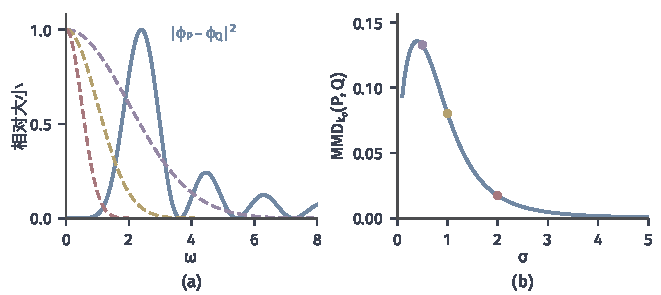
\includegraphics[width=112mm]{figures/07-probability/04-distribution-analysis/matplotlib/dcomp-mmd-spectrum/figure.pdf}
 \caption{高斯核MMD的频率图景，$P=\mathcal{N}(0,1)$，$Q=\operatorname{Unif}(-\sqrt3,\sqrt3)$。(a)蓝线是$\lvert\phi_P(\omega)-\phi_Q(\omega)\rvert^{2}$（除以最大值约$0.0679$）；虚线是频率权重$\exp(-\sigma^{2}\omega^{2}/2)$，紫、黄、红依次为$\sigma=0.5,1,2$。(b)$\operatorname{MMD}_{k_\sigma}(P,Q)$随$\sigma$的变化，三个点对应(a)中的三个带宽，数值约为$0.1329$，$0.0804$，$0.0174$。}
 \label{fig:dcomp-mmd-spectrum}
\end{BookInlineFigure}

特征核只保证“零值等价于分布相同”。一列分布的MMD趋于零能否推出弱收敛，是另一个问题，第~\ref{sec:dcomp-mmd-convergence}节专门讨论。
